\setAuthor{Jaan Kalda}
\setRound{lõppvoor}
\setYear{2014}
\setNumber{G 10}
\setDifficulty{10}
\setTopic{Geomeetriline optika}

\prob{Klaassilinder}
Klaassilindri välispinnal märgitakse markeriga punkt. Kui seda silindrit vaadata suurelt kauguselt (hulga suuremalt kui silindri raadius) nii, et punkt paistab läbi silindri selle sümmeetriateljel olevat, siis on lisaks näha veel kahte punkti kujutist. Üks kujutis on näha ühel ja teine teisel pool sümmeetriatelge. Kui silindrit keerata ümber oma sümmeetriatelje, siis teatud hetkel sulavad kaks punkti kujutist kokku ning kaovad ära. Kolmas kujutis jääb alles. Kui silindrit edasi keerata, siis hetkel, kui selle pöördenurk algasendi suhtes on \ang{15}, kaob ka kolmas kujutis, nõnda et markeriga tehtud punkti polegi enam näha. Kui suur on klaasi murdumisnäitaja?

\hint
Tähistame märgitud punkti $A$-ga ja silindri keskpunkti $O$-ga. Antud ülesande kontekstis tasub vaadelda funktsiooni $f(\alpha) = \delta$, mis kirjeldab punktist $A$ alguse saanud kiire silindrist väljumise nurka $\delta$ kiire $AO$ suhtes funktsioonina stardinurgast $\alpha$ kiire $AO$ suhtes. Silindri algasendit kirjeldab $f(\alpha) = 0$ kolme lahendiga. Lisaks on teada, et $f(\alpha) = \ang{15}$ on lahenditeta.

\solu
\begin{wrapfigure}{r}{0.35\textwidth}%
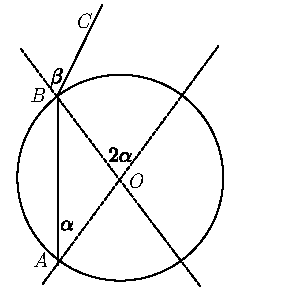
\includegraphics[trim = 0mm 0mm 12mm 0mm, clip, width=1\linewidth]{2014-v3g-10-silinder}
\end{wrapfigure}

Tähistame märgitud punkti $A$-ga ning murdugu sealt lähtunud kiir punktis $B$ nii, et suundub eemale läbi punkti $C$ (vt joonist).
Sihi $BC$ suunast kaugelt vaadatuna näeme tumeda punkti asukohana punkti $B$. Uurime, kuidas sõltub kiire $BC$ levikusuund, mida kirjeldame 
$AO$ ja $BC$ vahelise nurga $2\alpha-\beta$ abil, kiire algsest levikusuunast $\alpha$:
$$2\alpha-\beta= 2\alpha-\arcsin (n\sin\alpha).$$

Silindri algasendi korral $2\alpha-\arcsin (n\sin\alpha) =0$, mille üks lahend $\alpha=0$ annab keskmise näiva punkti
ning kaks külgmist tumedat punkti vastavad võrrandi $\sin(2\alpha)=n\sin\alpha$ ülejäänud lahenditele vahemikus $-45^\circ <\alpha<45^\circ$.
Kui pöörata nüüd silindrit nurga $\delta$ võrra, siis vastavad näivad punktid võrrandi 
$$2\alpha-\arcsin (n\sin\alpha) =\delta$$
lahenditele. Võrrandi vasakul pool on funktsioon, mis väikeste nurkade puhul käitub kui $(2-n)\alpha$; suuremate nurkade puhul teise liidetava suhteline mõju kasvab.
Seega juhul $2>n$, on tegemist väikeste nurkade puhul kasvava funktsiooniga, mis läheb suuremate nurkade puhul üle kahanevaks;
juhul $2<n$ on see aga monotoonselt kahanev funktsioon. Kuivõrd $\delta=0$ puhul on kolm lahendit, siis peab olema tegemist esimese juhtumiga, $2>n$.
Nende pöördenurkade $\delta$ puhul, mis on suuremad selle funktsiooni lokaalsest maksimumist, on võrrandil vaid üks lahend.
Funktsioon saavutab globaalse maksimumi täieliku sisepeegelduse piirjuhul 
$$n\sin\alpha=-1,$$
mis annab pöördenurga
$$90^\circ-2\arcsin \frac 1n=\SI{15}{}^\circ\Rightarrow n=1/\sin \ang{37,5} = \SI{1,64}{}.$$

\probeng{Glass cylinder}
A point is marked on the outer surface of a glass cylinder. If that cylinder is observed at a great distance (much bigger than the radius of the cylinder), so that through the cylinder the point seems to be on the symmetry axis, then two additional images of the point can be seen. One point can be seen on one side of the symmetry axis, the second on the other side. If the cylinder were turned around its symmetry axis then at a particular moment those two points would merge together and disappear. The third image stays. If continuing to turn the cylinder, then at the moment when the angle of rotation with respect to the initial position is $\ang{15}$, the third image would disappear so that the marked point would not be seen anymore. How big is the refractive index of the glass?

\hinteng
Let us label the marked point as $A$ and the center of the cylinder as $O$. It is useful to consider the function $f(\alpha) = \delta$, which describes the departure angle, $\delta$, of a ray entering the cylinder at the point $A$ as a function of the entrance angle $\alpha$, where all the angles are measured with respect to the ray $AO$. The initial position of the cylinder is described by $f(\alpha) = 0$ with three solutions. In addition it is known that $f(\alpha) = \ang{15}$ is without solutions.

\solueng
\begin{wrapfigure}{r}{0.35\textwidth}%
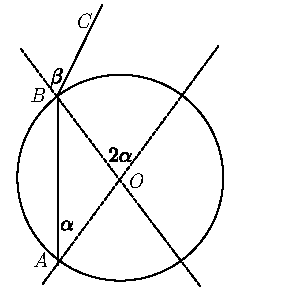
\includegraphics[trim = 0mm 0mm 12mm 0mm, clip, width=1\linewidth]{2014-v3g-10-silinder}
\end{wrapfigure}
Let the marked point be $A$ and let us assume that the ray going through it refracts in a point $B$ so that it is directed away through a point $C$ (see figure). Observing from far away from the direction of $BC$ we see the location of the dark point to be the point $B$. Let us see how the travel direction of the ray $BC$, that is described with the angle between $AO$ and $BC$, $2\alpha-\beta$, depends on the initial travel direction $\alpha$ of the ray:
$$2\alpha-\beta= 2\alpha-\arcsin (n\sin\alpha).$$
For the initial position of the cylinder $2\alpha-\arcsin (n\sin\alpha) =0$. One of its solution $\alpha=0$ gives us the middle virtual point and the two outer dark points meet the solutions of the equation $\sin(2\alpha)=n\sin\alpha$ in the interval $-45^\circ <\alpha<45^\circ$. If the cylinder were now turned by an angle $\delta$ then the virtual points meet the solutions of the equation
$$2\alpha-\arcsin (n\sin\alpha) =\delta$$
On the left side of the equation there is a function that in the case of small angles acts as $(2-n)\alpha$; in the case of bigger angles the relative effect of the second addend increases. Therefore if $2>n$ we are dealing with an increasing function in the case of small angles, this function starts to decrease in the case of bigger angles; if $2<n$ it is, however, a monotonically decreasing function. Since in the case of $\delta=0$ there are three solutions then we have to be dealing with the first case, $2>n$. In the case of such rotation angles $\delta$ that are bigger from the relative maximum of this function the equation only has one solution. The function reaches the absolute maximum in the limit case of a total internal reflection
$$n\sin\alpha=-1,$$
that gives us the rotation angle 
$$90^\circ-2\arcsin \frac 1n=\SI{15}{}^\circ\Rightarrow n=1/\sin \ang{37,5} = \SI{1,64}{}.$$
\probend